\subsection{Conflict Resolution}


\begin{frame}[fragile]
  \frametitle{Merge Conflicts}
  
  \begin{center}
    \Large Don't Panic!
  \end{center}

  \begin{itemize}
  \item 
    Merge conflicts happen if there are overlapping edits.
  \item 
    Resolving them is common and easy.
  \end{itemize}
  
  Example:
  \begin{latexCode}
    \begin{equation}
      \label{eq:quad}
      x = \frac{-b+-\sqrt{b^2-4ac}}{2a}
    \end{equation}
    are the two roots of the quadratic equation.
  \end{latexCode}
  
\end{frame}



\begin{frame}[fragile]
  
  On the flight to a conference I change this to
  \begin{latexCode}
    \begin{equation}
      \label{eq:quad}
      x_{1,2} = \frac{-b+-\sqrt{b^2-4ac}}{2a}
    \end{equation}
    are the two roots of the quadratic equation.
  \end{latexCode}
  \bigskip
  \pause
  
  While I'm still in the air, Jennifer corrects
  \begin{latexCode}
    \begin{equation}
      \label{eq:quad}
      x = \frac{-b\pm\sqrt{b^2-4ac}}{2a}
    \end{equation}
    are the two roots of the quadratic equation.
  \end{latexCode}
  and pushes it to our common remote repository.
  
\end{frame}


\begin{frame}[fragile]
  \frametitle{Reconnecting...}
  
  When I try to push my commit, git rightfully refuses:
  \begin{tinyshell}
[vbraun@laptop]$ git push
To git@github.com:vbraun/talk-git-sage-workflow.git
 ! [rejected]        quadratic_equation -> quadratic_equation (non-fast-forward)
error: failed to push some refs to 'git@github.com:vbraun/talk-git-sage-workflow.git
hint: Updates were rejected because the tip of your current branch is behind
hint: its remote counterpart. Merge the remote changes (e.g. 'git pull')
hint: before pushing again.
hint: See the 'Note about fast-forwards' in 'git push --help' for details.
  \end{tinyshell}  %$

  The \cmd{git status} says the same thing:
  \begin{smallshell}
[vbraun@laptop]$ git status
# On branch quadratic_equation
# Your branch and 'origin/quadratic_equation' have diverged,
# and have 1 and 1 different commit each, respectively.
#   (use "git pull" to merge the remote branch into yours)
#
nothing to commit, working directory clean
  \end{smallshell}%$

\end{frame}


\begin{frame}[fragile]  
  
  I have to first pull\footnote{That is, download and merge}
  Jennifer's overlapping edit:
  \begin{smallshell}
[vbraun@laptop]$ git pull
Auto-merging example/quadratic_equation.tex
CONFLICT (content): Merge conflict in 
                    example/quadratic_equation.tex
Automatic merge failed; fix conflicts and then commit the 
result.
  \end{smallshell} %$
  \medskip
  \pause

  The file now looks like this:
  \begin{latexCode}
      \begin{equation}
    \label{eq:quad}
<<<<<<< HEAD
    x_{1,2} = \frac{-b+-\sqrt{b^2-4ac}}{2a}
=======
    x = \frac{-b\pm\sqrt{b^2-4ac}}{2a}
>>>>>>> d0615cf02b5615a07c34633dabaf3c0eb57cac7a
  \end{equation}
  are the two roots of the quadratic equation.
  \end{latexCode}
\end{frame}
   

\begin{frame}
  \frametitle{Resolving the Conflict}

  \begin{itemize}
  \item Open the file in your favorite editor and fix, or
  \item Use a specialized program (I like \cmd{meld}): \cmd{git mergetool}\\
    \medskip

    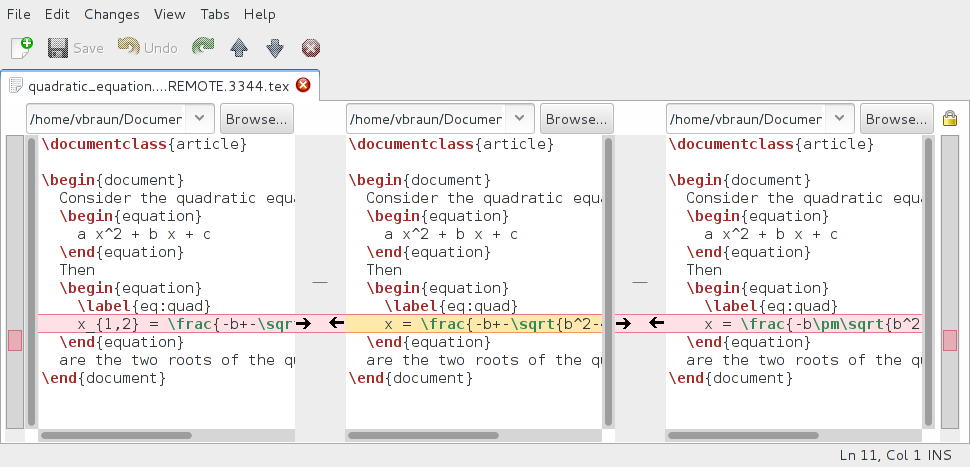
\includegraphics[width=\linewidth]{images/mergetool_meld}
  \end{itemize}
\end{frame}


\begin{frame}
  \frametitle{Finishing Up}

  \begin{itemize}
  \item When you are finished resolving the conflict, just commit:\\
    \cmd{git add quadratic\_equation.tex}\\
    \cmd{git commit -m 'merged Jennifers TeX fix'}
  \item Now, git lets me push to the remote repository.
  \item When Jennifer pulls from the remote later, she gets my change
    and my resolution of the conflict.
  \item To abort the merge:\\
    \cmd{git merge --abort}    
  \end{itemize}
\end{frame}


{
  \usebackgroundtemplate{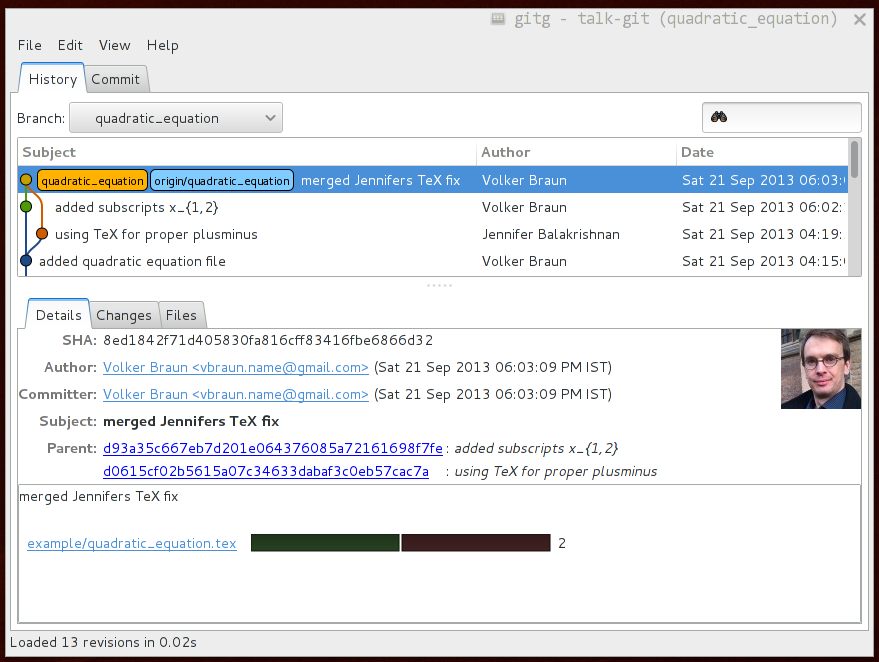
\includegraphics[width=\paperwidth]{images/after_merge}}
  \begin{frame}[plain]
  \end{frame}
}


%%% Local Variables:
%%% TeX-master: "talk.tex"
%%% eval: (TeX-PDF-mode 1)
%%% End:
